\documentclass{article}
\usepackage{graphicx}
\usepackage{float}
\usepackage{titlesec}
\usepackage{datetime}
\usepackage{geometry}
\usepackage{minted}
\usepackage{placeins}
\usepackage{caption}
\usepackage[document]{ragged2e}
\usepackage[hidelinks]{hyperref}
\usepackage{enumitem}
\geometry{
 a4paper,
 left=25mm,
 top=25mm,
 }
\captionsetup{hypcap=false} 
\newdateformat{daymonthyear}{\THEDAY .\THEMONTH .\THEYEAR}
\title{
  \centering
  
\includegraphics[width=\textwidth]{images/logo_PWr_kolor_poziom.png}\\
  \fontsize{28pt}{30pt}\selectfont Sprawozdanie 5\\
  }
\author{Krzysztof Zalewa}
\date{\daymonthyear\today}
\renewcommand*\contentsname{Spis treści}
\renewcommand{\figurename}{Rysunek}
\renewcommand{\listingscaption}{Skrypt}
\begin{document}
    \maketitle
    \pagebreak
    \tableofcontents
    \FloatBarrier
    \raggedright
    \section{Cel skryptu}
        Cele zajęć laboratoryjnych było przygotowanie prostego czatu przy użyciu pythona.
        Całe zadanie podzielone jest na dwie części serwer i klienta. Serwer obsługuje połączenia z klientami.
        Oraz przesyła między nimi wiadomości.
        Klienci to okna w terminalu obsługiwane przez użytkowników pozwalające na wyświetlanie i wysyłanie wiadomości.

        Zadanie wykonano przy użyciu bibliotek socket(połączenia) oraz threading(wielowątkowość by połączyć wielu klientów na raz
        oraz by odbieranie i wysyłanie mogło się dziać równocześnie)

    \section{Opis skryptu}
      
        \begin{frame}
            \scriptsize
            \inputminted[
                style={vs},
                breaklines,
                breakanywhere, 
                linenos, 
                tabsize=4 
            ]{python}{./server.py}
            \vspace{1em}
            \captionof{listing}{Kod servera}
            \label{lst:script_1}
        \end{frame}
      
        \begin{frame}
            \scriptsize
            \inputminted[
                style={vs},
                breaklines,
                breakanywhere, 
                linenos, 
                tabsize=4 
            ]{python}{./client.py}
            \vspace{1em}
            \captionof{listing}{Kod klienta}
            \label{lst:script_2}
        \end{frame}

    \section{Wnioski}
        Kod działa poprawnie.
        Po uruchomieniu serwera klienci mogą się do niego połączyć.
        A wiadomości wyświetlanie są poprawnie
        \begin{figure}[ht]
            \centering
            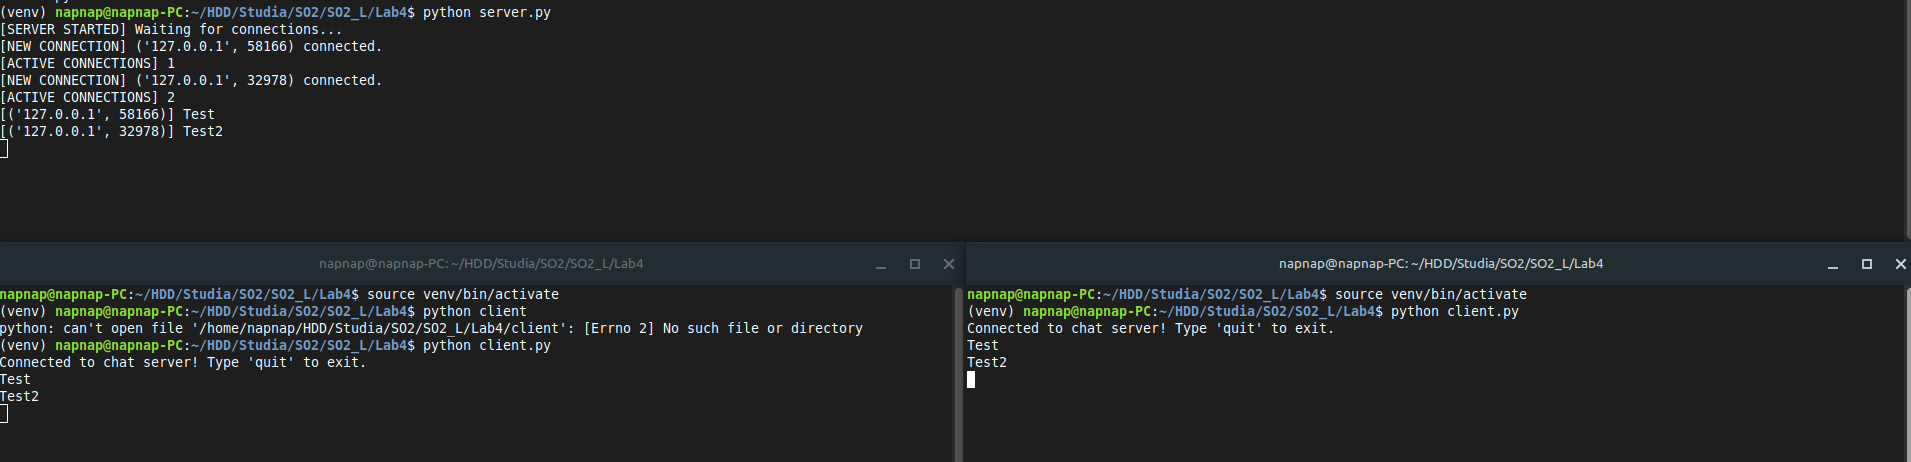
\includegraphics[width=\textwidth]{images/image.png}
            \caption{Przykład działania. Wiadomość "Test" wysłana z terminala po prawej, "Test1" po lewej}
            \label{fig:run_succes}
        \end{figure}

\end{document}